%% Appendix: per-architecture playbook. Old \S4.2 (lever), \S4.3 (merge absorption) and R3
%% (lever ablation) moved here verbatim in the 2026-10-10 restructure. The merge-absorption
%% measurements come from a gpt-oss-120b run that is not otherwise reported in this paper.
\section{Per-architecture playbook}
\label{app:playbook}

\subsection{Merge absorption: when the install does not survive being served}
\label{sec:merge}

On a fused-expert mixture-of-experts model at rank 16, the adapter's per-element weight changes are
smaller than the step that bf16 storage can represent, so merging the adapter into the weights
rounds much of the install away while still changing the model's outputs; the merged model is
neither the base nor the trained model. We observed this on a gpt-oss-120b run that is not
otherwise reported here. The rule we draw from it: on such models, raise the rank until the changes
clear the storage step, or ship the adapter rather than merged weights. On the models we release
merged, merged weights and adapter agree (\S\ref{sec:cross}).

\subsection{Lever ablation on Qwen3-30B-A3B}
\label{sec:lever}

When you fine-tune with LoRA, you choose which parts of the network the adapter is allowed to
change; we call that choice the lever. On a dense model there is nothing to decide. On a
mixture-of-experts model like Qwen3-30B-A3B there are three kinds of parts: the attention layers,
the 128 expert MLPs, and the router that decides which experts handle each token. To find out which
parts the adapter needs to reach, we trained the same base on the same corpus four times, changing
only the lever (same v1 corpus, same A3 recipe, one serving stack, every answer parseable in every
arm). Table~\ref{tab:lever} and Figure~\ref{fig:p3} give the result. The practical rules we follow are:

\begin{description}
  \item[Dense.] Default. All linear projections; merge and ship merged weights.
  \item[MoE with per-expert \texttt{nn.Linear} modules.] Use the \emph{full} lever (attention plus
  expert MLPs) and never train the router. The router is a discrete assignment mechanism;
  adapting it changes which experts see which tokens, and the one arm in our record that included the
  router (\texttt{mlp.gate}) cost $-22$\,pp MMLU. We flag below that the attribution of that cost
  \emph{to the router specifically} is an inference from a different stack and era, not a
  demonstration (\S\ref{sec:lever}).
  \item[MoE with fused / quantized expert slabs.] Transformers 5.x fuses experts into stacked 3-D
  \texttt{nn.Parameter}s, which bitsandbytes cannot 4-bit quantize, so LoRA must reach them through
  the \texttt{target\_parameters} path. That path buys four problems at once: a per-forward dense
  delta materialization (7.91\,GiB fp32 on gpt-oss-120b, which makes adapter-mode evaluation cost
  $\approx$10\,min per cell on 8$\times$H100), routing coverage (top-4 of 128 means a small corpus
  trains whichever experts it happens to route to), a dropout constraint, and the merge-absorption
  problem of Appendix~\ref{sec:merge}. Prefer attention-only targets and \textbf{ship the adapter, not merged weights}.
\end{description}

\begin{table}[t]
\centering\footnotesize
\caption{Lever ablation on Qwen3-30B-A3B. Breaking \auc{} over L0--L5 and breaking rate at the
maximum-pressure rung L5 (lower is better); MMLU change in percentage points on a 50-item probe.
The router was never adapted. Base MMLU here is the earlier $44/50$ probe run (see the footnote in
\S\ref{sec:cross}).}
\label{tab:lever}
\begin{tabular}{@{}llccc@{}}
\toprule
Arm & Parts the adapter may change & Breaking \auc{} & Breaking at L5 & MMLU change \\
\midrule
base (no training) & none & 0.196 & 0.773 & reference (88.0\%) \\
full lever & attention + all experts & \textbf{0.000} & \textbf{0.000} & not measured \\
attention only & attention & 0.036 & 0.182 & $+2$ \\
early experts & attention + experts in layers 0--15 & 0.077 & 0.227 & $+2$ \\
late experts & attention + experts in layers 32--47 & 0.073 & 0.273 & $-4$ \\
\bottomrule
\end{tabular}
\end{table}

\begin{figure}[p]
\centering
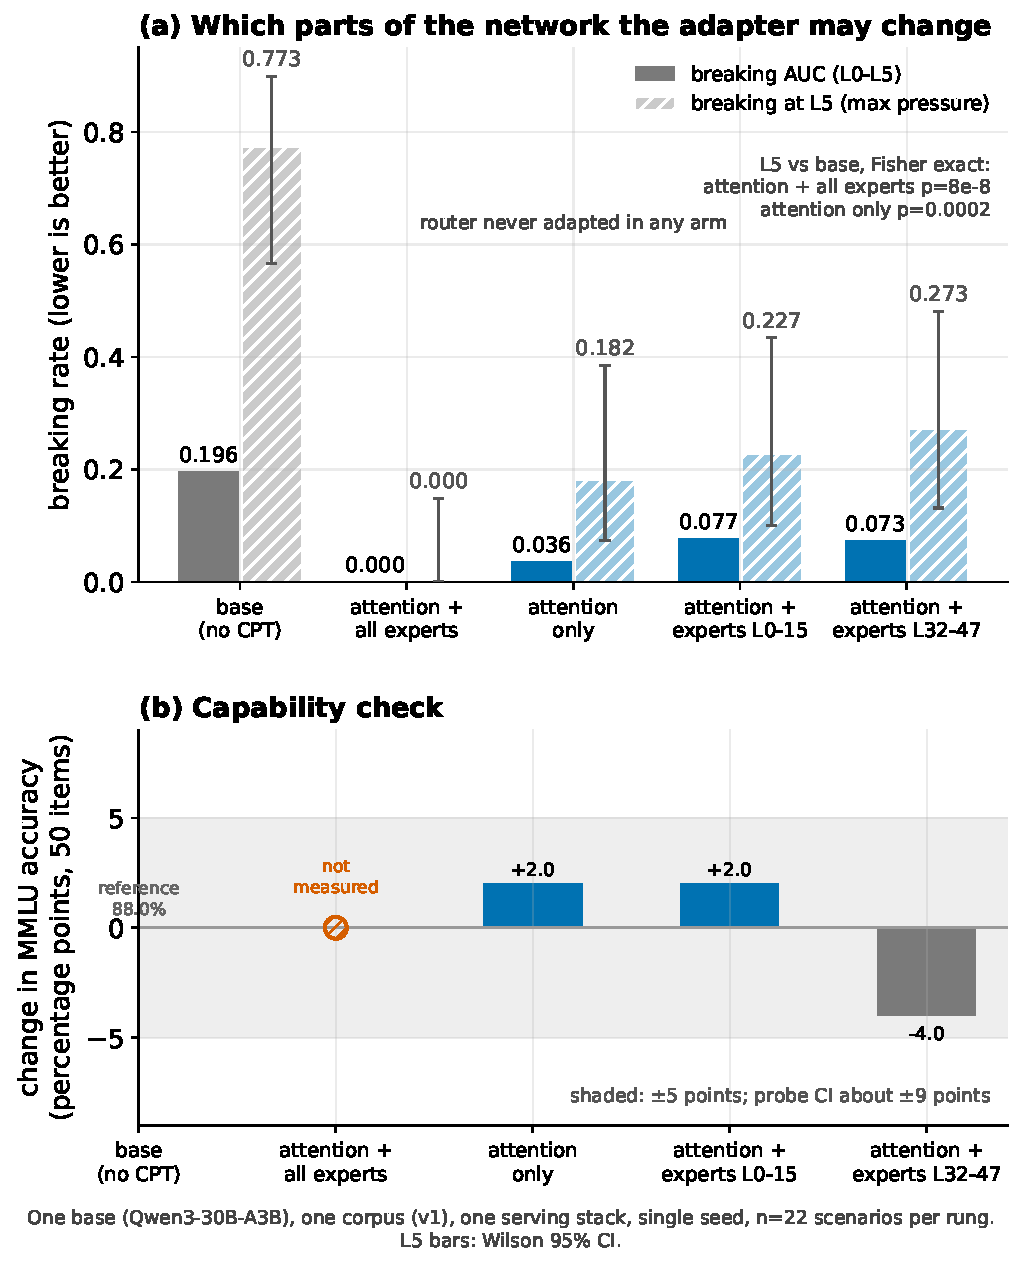
\includegraphics[width=0.9\textwidth]{P3_lever_ablation.pdf}
\caption{Which parts of the network the adapter may change, on Qwen3-30B-A3B. \textbf{(a)}
Breaking \auc{} over L0--L5 (solid) and breaking at the maximum-pressure rung L5 (hatched); lower
is better; $n{=}22$ scenarios per rung. Only the arm that adapts attention and all experts reaches
zero at L5. L5 bars carry Wilson 95\% intervals. \textbf{(b)} Change in MMLU
accuracy in percentage points; the full-lever arm's MMLU was not measured. The router was never
adapted.}
\label{fig:p3}
\end{figure}

We draw three conclusions from this, and note a fourth that we cannot draw.

First, letting the adapter reach attention plus all experts is what works: breaking goes to zero
at every pressure level, including L5.

Second, attention only is a usable fallback. It gets most of the way (\auc{} $0.196 \to 0.036$) at
no cost on MMLU, but at maximum pressure the model still breaks about one time in five (L5
$0.182$). This matters because on some MoE models the experts are stored in a fused or quantized
form that LoRA cannot reach (FP4/FP8 routed experts, MXFP4 slabs), so attention is the only lever
available; this arm shows the install is still worth attempting there.

Third, the router should not be adapted. We state this as a design rule rather than a measured
result: one older run that adapted the router lost 22 MMLU points, but it ran on a different
software stack with a different base anchor ($0.250$ vs.\ $0.196$), so we cannot attribute the loss
to the router alone. A matched run on the current stack would settle it and has not been done.

What we cannot conclude is anything about the two partial-expert arms. Both scored slightly worse
than attention only ($0.077$ and $0.073$ vs.\ $0.036$), which might suggest that adapting some
experts is worse than adapting none, but with 22 scenarios per rung and one seed these differences
amount to one scenario flipping at one rung, and the ordering is not even consistent across the
secondary metrics (the late arm's positive-sum rate, $0.925$, exceeds the early arm's $0.888$). We
offer them as hypotheses for replication.

\subsection{Recipe notes}
\label{app:recipe-notes}

The effective batch of 32 is enforced in code (\texttt{batch} $\times$ \texttt{grad\_accum} must
equal 32; micro-batching is not part of the recipe). Two optional levers of the companion paper,
Qi-style token weighting and a recovery stratum \citep{northen2026depth,qi2025safety}, were left
off so that the plainest recipe isolates what the corpus does. The released Qwen3-30B-A3B
``shallow'' adapter's \texttt{adapter\_config.json} lists
\texttt{target\_modules = [q,k,v,o,gate,up,down]\_proj} at $r{=}16$, $\alpha{=}32$ with
\texttt{target\_parameters} unset, i.e.\ attention plus per-expert MLPs with the router not
matched; the adapter-to-arm mapping for that release was originally inferred from upload timestamps.
